\documentclass[a4paper, amsfonts, amssymb, amsmath, reprint, showkeys, nofootinbib, twoside]{revtex4-1}
\usepackage[english]{babel}
\usepackage[utf8]{inputenc}
\usepackage[colorinlistoftodos, color=green!40, prependcaption]{todonotes}
\usepackage[pdftex, pdftitle={Article}, pdfauthor={Author}]{hyperref}
\usepackage{amsthm}
\usepackage{mathtools}
\usepackage{physics}
\usepackage{xcolor}
\usepackage{caption}
\usepackage{hyperref}
%\hypersetup{colorlinks=true, linkcolor=blue, urlcolor = blue}
\usepackage{amsmath}
\usepackage{amssymb}
\usepackage{graphicx}
\graphicspath{Images}
\usepackage[left=23mm,right=13mm,top=35mm,columnsep=15pt]{geometry} 
\usepackage{adjustbox}
\usepackage{placeins}
\usepackage[T1]{fontenc}
\usepackage{float}
%\usepackage{longtable}
\usepackage{csquotes}
\usepackage{refstyle}
\usepackage{lipsum}

\begin{document}

\title{Study of Hall effect in Semi-Conductors}
\author{Swaroop Ramakant Avarsekar}
\email{swaroop.avarsekar@niser.ac.in}
\affiliation{School of Physical Sciences, National Institute of Science Education and Research, HBNI, Jatni -752050, India}
\date{\today}
	
\begin{abstract}
Potential difference across the current carrying conductor when subjected to normal magnetic field is due to Hall effect. In this experiment,  we aim to determine the Hall coefficient of n type and p type semiconductors and study the variation of Hall coefficient with temperature. Hall coefficient of n type Ge is $R_H=-0.0787\pm0.0004 m^3/C$ and charge carrier density as $n=(7.93\pm0.04)\times10^{19}/m^3$ and for p type Ge $R_H=0.0122\pm0.0003 m^3/C$ and $n=(5.11\pm0.01)\times10^{20}/m^3$.
\end{abstract}
	
\keywords{Hall coefficient, Gaussmeter, Lorentz Force}
	
\maketitle

\section{Theory}
Hall effect is a phenomenon when a current carrying conductor/crystal where the direction of current is along x, with direction of magnetic field H from top gives the voltage across the ends 1 and 2 due to Hall effect, as shown in Figure(1). This magnetic field exerts a Lorentz force on charge carriers as given below:
\begin{equation}
	\bar{F}=e(\bar{v}\times\bar{H})
\end{equation}

where e is charge of electron, v is drift velocity of charge carriers, H is magnetic field applied. This Lorentz force drags the electrons and holes towards opposite ends of the crystal, resulting a electric field, called Hall field ($E_H$), opposite to Lorentz force. Deflection of charge carriers takes place until Hall field cancels the Lorentz Force giving rise to a potential difference, called Hall voltage ($V_H$) . 

\begin{figure}[H]
	\centering
	\includegraphics[scale=0.36]{1} 
	\caption{Hall effect in a crystal}
	\label{1}
\end{figure}

The field along y-axis is given by 
\begin{equation}
	E_m=vH=\mu E_x H
\end{equation}

This electric field is related to current density and conductivity as
\begin{equation}
	\sigma E_x=J_x
\end{equation}

The Hall coefficient $R_H$ is defined as 
\begin{equation}
	R_H=E_m/J_x H=\mu E_x /J_x=\mu/\sigma=1/ne
\end{equation}

The Hall voltage is proportional to 1/n and $ \mu =R_H \sigma $. Experimentally, the Hall coefficient is given by 
\begin{equation}
	R_H=\frac{V_y /b}{(I_x/bt)H}=V_y t/I_x H
\end{equation}

where b and t are width and thickness of the sample.

If voltage across the input is kept constant, then Hall angle as the ratio of applied and measured voltages.
\begin{equation}
	\phi=V_y/V_x=E_m b/E_x I=\mu b H/l 
\end{equation}

where l is the length of the crystal. 

When both type of charge carriers are present, hall coefficient is given by 
\begin{equation}
	R_H=\frac{\mu_h^2p-\mu_e^2n}{e(\mu_h^2p+\mu_e^2n)}
\end{equation}

Since the mobilities $\mu_h$ and $\mu_e$ are not constants but functions of T, the Hall coefficient above equation, is also a function of T and it may become zero and even change sign. In general, $\mu_e>\mu_h$, so that inversion may happen only if p > n; thus Hall coefficient inversion is characteristic
of only p-type semiconductors.

\section{Experiment \& Analysis}
The experimental setup is as shown in figure (2).
\begin{figure}[H]
	\centering
	\includegraphics[scale=0.1]{e} 
	\caption{Experimental setup in laboratory}
	\label{2}
\end{figure}

The magnetic field is calibrated with applied voltage. Measure the Hall voltage with the probe current for n type and p type Ge. Then calculate Hall coefficient at the room temperature.Keeping fixed probe current, vary the heater current and record the Hall voltage. The sign of Hall voltage changes for p type Ge.   

\begin{table}[H]
	\centering
	\caption{Magnetic Field Calibration}
	\label{t1}
		\begin{tabular}{|r|r|}
			\hline
			\multicolumn{1}{|l|}{Current (A)} & \multicolumn{1}{l|}{\begin{tabular}[c]{@{}l@{}}Magnetic \\ Field (Gauss)\end{tabular}} \\ \hline
			0.03 & 24   \\ \hline
			0.06 & 43   \\ \hline
			0.07 & 57   \\ \hline
			0.09 & 68   \\ \hline
			0.11 & 85   \\ \hline
			0.13 & 107  \\ \hline
			0.27 & 224  \\ \hline
			0.38 & 320  \\ \hline
			0.5  & 434  \\ \hline
			0.6  & 522  \\ \hline
			0.77 & 674  \\ \hline
			0.97 & 854  \\ \hline
			1.12 & 991  \\ \hline
			1.32 & 1173 \\ \hline
			1.55 & 1383 \\ \hline
			1.93 & 1718 \\ \hline
			2.22 & 1989 \\ \hline
			2.39 & 2120 \\ \hline
			2.57 & 2280 \\ \hline
			2.76 & 2440 \\ \hline
			2.97 & 2630 \\ \hline
			3.25 & 2900 \\ \hline
			3.47 & 3040 \\ \hline
			3.74 & 3530 \\ \hline
		\end{tabular}
\end{table}

\begin{table}[H]
	\centering
	\caption{Probe current Versus Hall voltage for n-Ge; Constant current source= 3 A}
	\label{t2}
		\begin{tabular}{|r|r|r|r|}
			\hline
			\multicolumn{1}{|l|}{\begin{tabular}[c]{@{}l@{}}Probe \\ Current (mA)\end{tabular}} &
			\multicolumn{1}{l|}{\begin{tabular}[c]{@{}l@{}}Hall \\ Voltage (mV)\end{tabular}} &
			\multicolumn{1}{l|}{\begin{tabular}[c]{@{}l@{}}Hall Voltage \\ Outside (mV)\end{tabular}} &
			\multicolumn{1}{l|}{\begin{tabular}[c]{@{}l@{}}Corrected Hall\\  Voltage (mV)\end{tabular}} \\ \hline
			4.6  & -197.1 & 4.1 & -193   \\ \hline
			4.37 & -189.4 & 3.3 & -186.1 \\ \hline
			4.14 & -180.3 & 3.1 & -177.2 \\ \hline
			3.92 & -170   & 3   & -167   \\ \hline
			3.71 & -161.8 & 3.3 & -158.5 \\ \hline
			3.47 & -151.7 & 2.7 & -149   \\ \hline
			3.31 & -146.3 & 2.9 & -143.4 \\ \hline
			3.01 & -132.8 & 2.6 & -130.2 \\ \hline
			2.81 & -125   & 2.3 & -122.7 \\ \hline
			2.56 & -113.4 & 4.2 & -109.2 \\ \hline
			2.29 & -101.2 & 2   & -99.2  \\ \hline
			2.01 & -89.9  & 1.5 & -88.4  \\ \hline
			1.79 & -80.4  & 1.5 & -78.9  \\ \hline
			1.56 & -69.6  & 1.3 & -68.3  \\ \hline
			1.19 & -53.6  & 1.2 & -52.4  \\ \hline
			0.99 & -44.6  & 1   & -43.6  \\ \hline
			0.77 & -34.4  & 0.8 & -33.6  \\ \hline
			0.49 & -21.7  & 0.5 & -21.2  \\ \hline
			0.14 & -6.2   & 0.2 & -6     \\ \hline
			0.07 & -3.2   & 0.1 & -3.1   \\ \hline
		\end{tabular}
\end{table}

\begin{figure}[H]
	\centering
	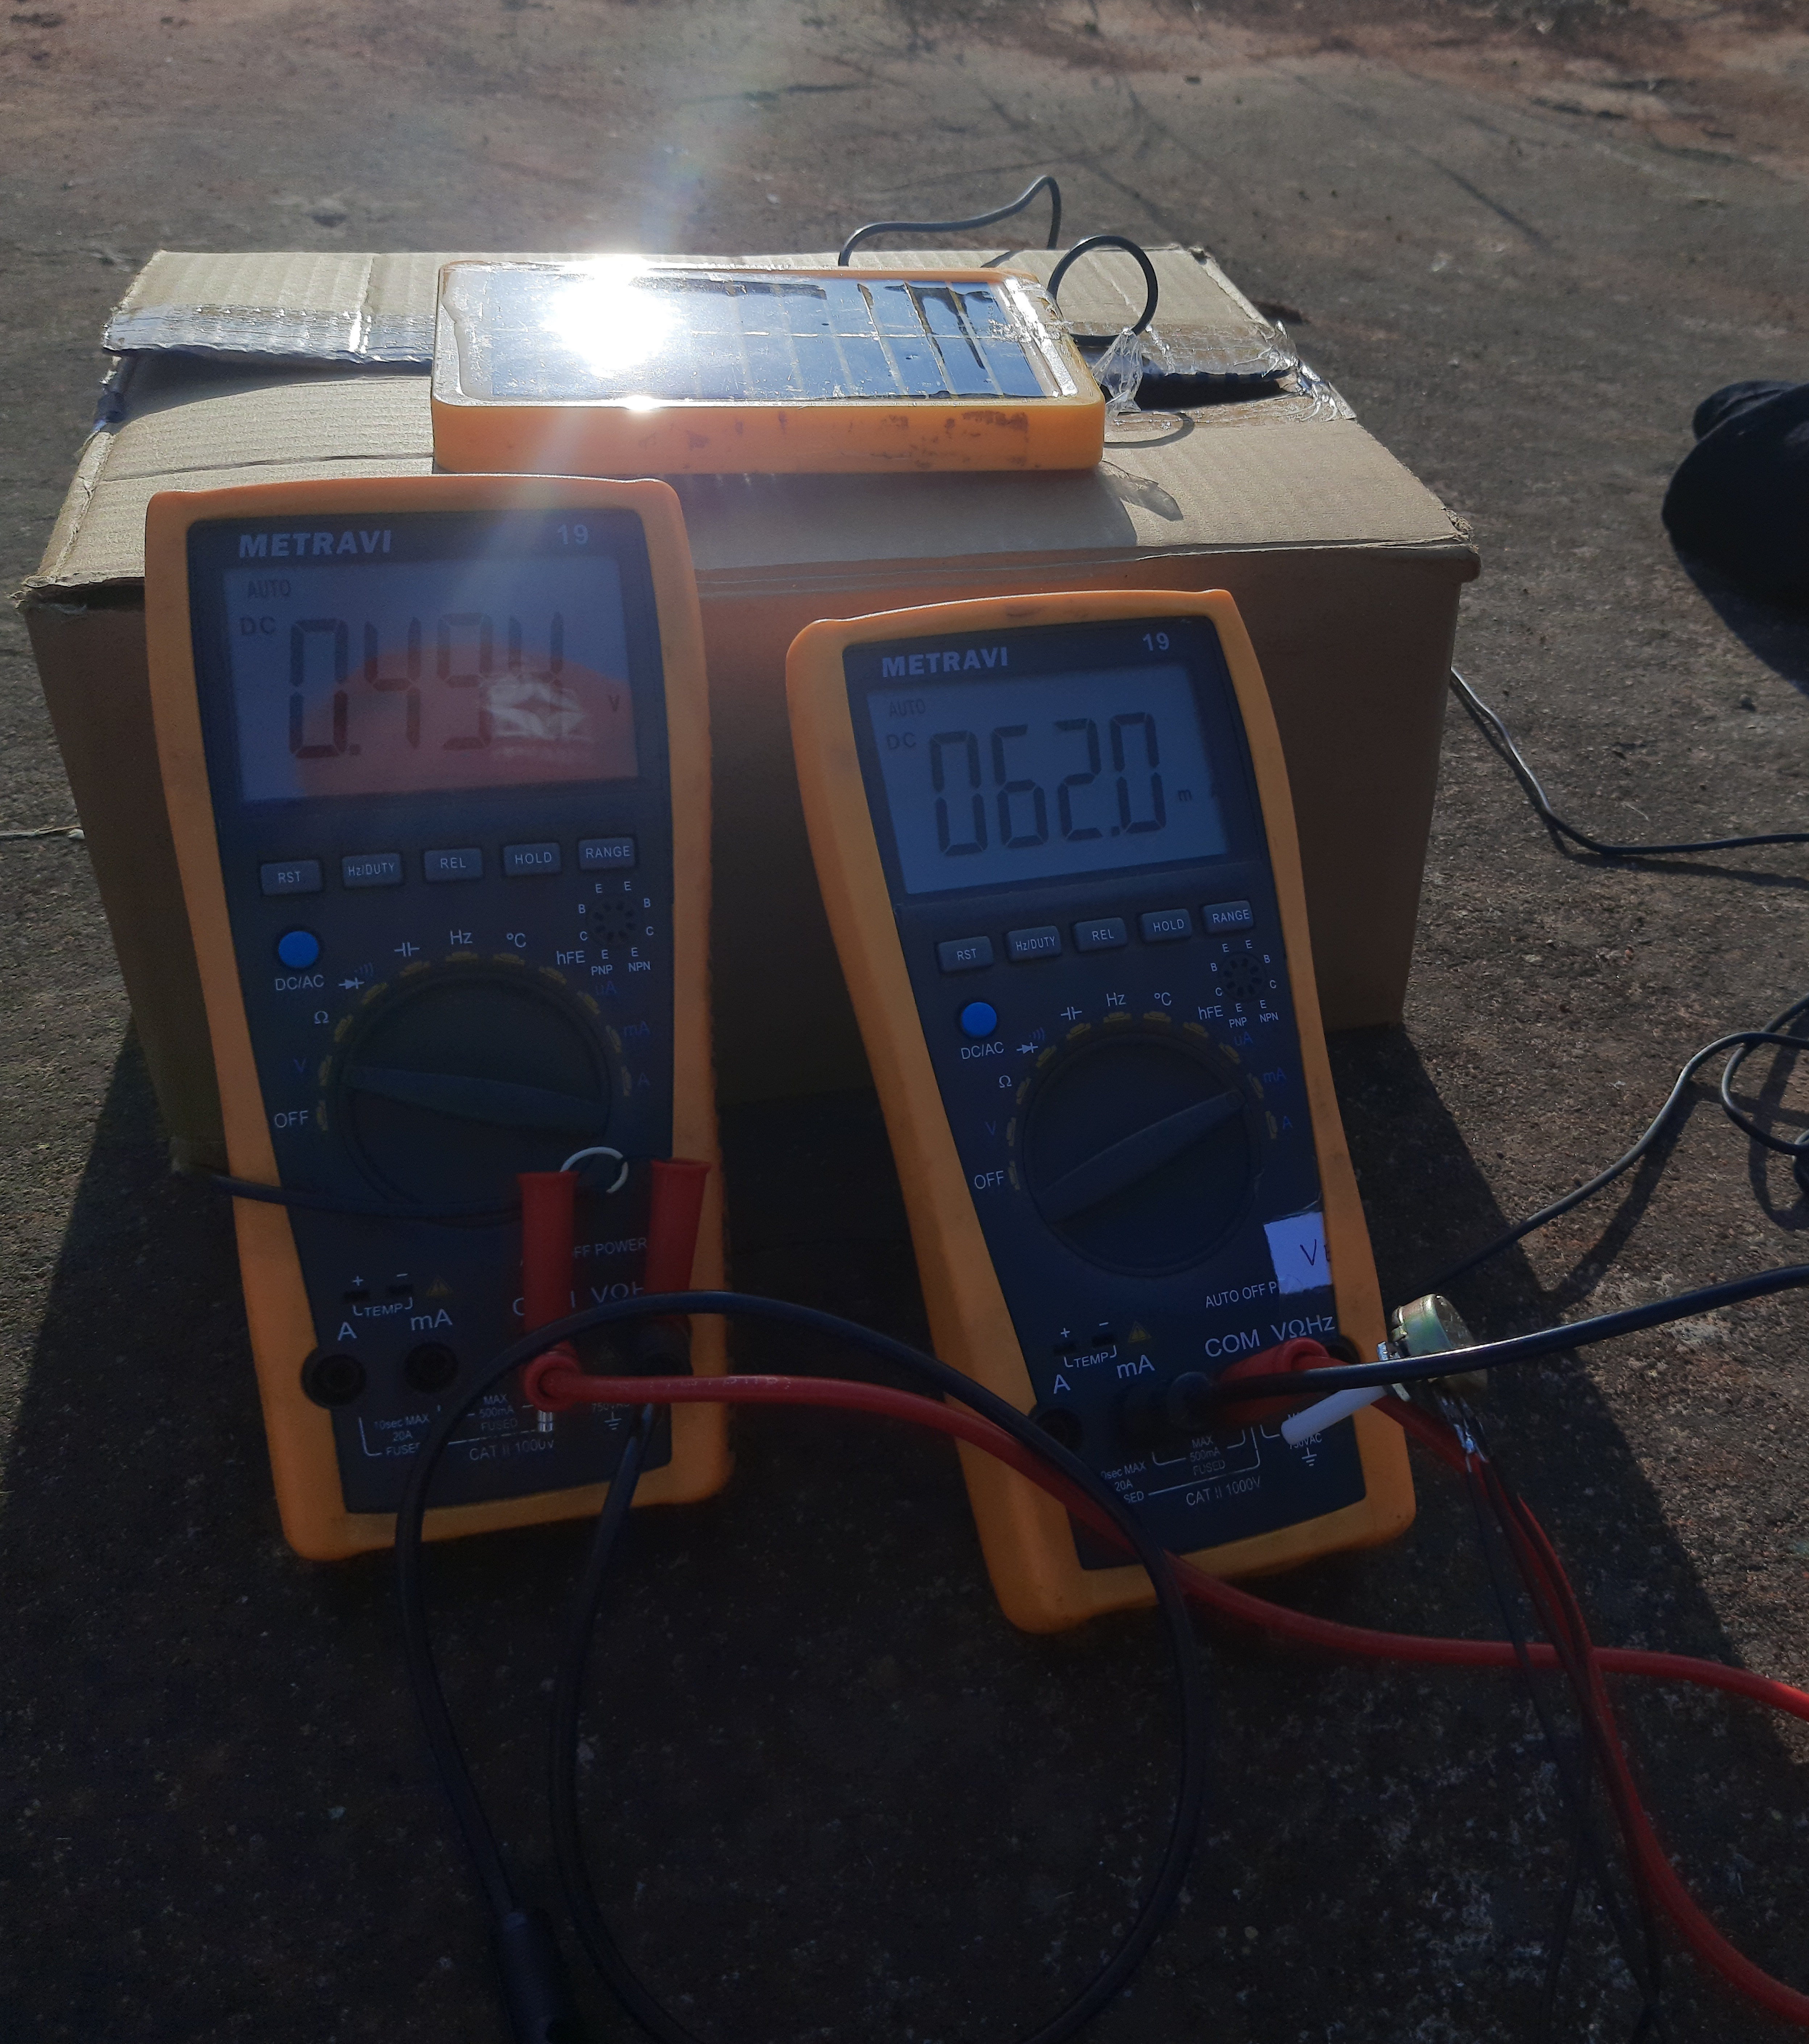
\includegraphics[scale=0.4]{2} 
	\caption{Calibration of magnetic field with applied voltage}
	\label{3}
\end{figure}

\begin{figure}[H]
	\centering
	\includegraphics[scale=0.55]{3} 
	\caption{Plot of Probe current versus Hall Voltage for n-Ge}
	\label{4}
\end{figure}

\begin{figure}[H]
	\centering
	\includegraphics[scale=0.55]{4} 
	\caption{Plot of Probe current versus Hall Voltage for p-Ge}
	\label{5}
\end{figure}

\begin{figure}[H]
	\centering
	\includegraphics[scale=0.55]{5} 
	\caption{Plot of Temperature versus Hall coefficient for p-Ge}
	\label{6}
\end{figure}

\begin{table}[H]
	\centering
	\caption{Probe current Versus Hall voltage for p-Ge; Constant current source= 3 A}
	\label{t5}
		\begin{tabular}{|r|r|r|r|}
			\hline
			\multicolumn{1}{|l|}{\begin{tabular}[c]{@{}l@{}}Probe \\ Current (mA)\end{tabular}} &
			\multicolumn{1}{l|}{\begin{tabular}[c]{@{}l@{}}Hall\\ Voltage (mV)\end{tabular}} &
			\multicolumn{1}{l|}{\begin{tabular}[c]{@{}l@{}}Hall Voltage \\ Outside (mV)\end{tabular}} &
			\multicolumn{1}{l|}{\begin{tabular}[c]{@{}l@{}}Corrected Hall \\ Voltage (mV)\end{tabular}} \\ \hline
			0.42  & 4     & 0.07 & 3.93 \\ \hline
			1.17  & 9.9   & 2.3  & 7.6  \\ \hline
			2.11  & 16.6  & 4.1  & 12.5 \\ \hline
			2.55  & 21.5  & 5.1  & 16.4 \\ \hline
			2.81  & 24.3  & 5.4  & 18.9 \\ \hline
			2.77  & 21.2  & 5.3  & 15.9 \\ \hline
			3     & 27.1  & 5.8  & 21.3 \\ \hline
			3.21  & 28.3  & 6.2  & 22.1 \\ \hline
			3.73  & 30.2  & 6.9  & 23.3 \\ \hline
			3.95  & 33.5  & 7.5  & 26   \\ \hline
			4.17  & 34.5  & 9.1  & 25.4 \\ \hline
			3.52  & 33.1  & 7.9  & 25.2 \\ \hline
			4.34  & 34    & 9.4  & 24.6 \\ \hline
			5.5   & 46.6  & 11.8 & 34.8 \\ \hline
			5.71  & 47    & 12.3 & 34.7 \\ \hline
			5.98  & 47.4  & 12.9 & 34.5 \\ \hline
			6.27  & 61.8  & 13.4 & 48.4 \\ \hline
			6.3   & 57.6  & 13.7 & 43.9 \\ \hline
			6.35  & 59.6  & 14.2 & 45.4 \\ \hline
			6.9   & 52.8  & 13.8 & 39   \\ \hline
			7.2   & 58.6  & 14.6 & 44   \\ \hline
			7.37  & 66.6  & 15   & 51.6 \\ \hline
			8.26  & 69.3  & 16.2 & 53.1 \\ \hline
			8.4   & 70.6  & 16.6 & 54   \\ \hline
			9.24  & 78.5  & 18.5 & 60   \\ \hline
			10.05 & 88.7  & 22.8 & 65.9 \\ \hline
			10.52 & 93.1  & 25.7 & 67.4 \\ \hline
			11.75 & 103.6 & 29.4 & 74.2 \\ \hline
			12.06 & 117.4 & 32.1 & 85.3 \\ \hline
		\end{tabular}
\end{table}

\begin{table}[H]
	\centering
	\caption{Temperature dependence of Hall Coefficient with p type Ge} \text{Constant current=2.22 A, Probe Current : 4 mA}
	\label{t6}
	\resizebox{\columnwidth}{!}{%
		\begin{tabular}{|r|r|r|r|r|r|r|r|}
			\hline
			\multicolumn{1}{|l|}{S No} &
			\multicolumn{1}{l|}{\begin{tabular}[c]{@{}l@{}}Heater \\ Current (mA)\end{tabular}} &
			\multicolumn{1}{l|}{\begin{tabular}[c]{@{}l@{}}Thermo \\ Emf (mV)\end{tabular}} &
			\multicolumn{1}{l|}{\begin{tabular}[c]{@{}l@{}}Temperature\\ ($^{\circ}C$)\end{tabular}} &
			\multicolumn{1}{l|}{\begin{tabular}[c]{@{}l@{}}Hall \\ Voltage (mV)\end{tabular}} &
			\multicolumn{1}{l|}{\begin{tabular}[c]{@{}l@{}}Residual \\ Voltage (mV)\end{tabular}} &
			\multicolumn{1}{l|}{\begin{tabular}[c]{@{}l@{}}Corrected Hall\\ Voltage (mV)\end{tabular}} &
			\multicolumn{1}{l|}{\begin{tabular}[c]{@{}l@{}}Hall coefficient \\ ($m^3/C$)\end{tabular}} \\ \hline
			1  & 0    & 0    & 26  & 34.1 & 9.5  & 24.6 & 0.00002785  \\ \hline
			2  & 100  & 0.03 & 27  & 36.5 & 10.2 & 26.3 & 0.00002978  \\ \hline
			3  & 200  & 0.16 & 31  & 33.6 & 9.9  & 23.7 & 0.00002683  \\ \hline
			4  & 300  & 0.38 & 36  & 36.3 & 10.1 & 26.2 & 0.00002966  \\ \hline
			5  & 400  & 0.63 & 42  & 34.1 & 9.2  & 24.9 & 0.00002819  \\ \hline
			6  & 500  & 1    & 51  & 27.6 & 5.7  & 21.9 & 0.00002479  \\ \hline
			7  & 550  & 1.23 & 57  & 26.4 & 7.4  & 19   & 0.00002151  \\ \hline
			8  & 600  & 1.43 & 62  & 21.2 & 6    & 15.2 & 0.00001721  \\ \hline
			9  & 650  & 1.63 & 66  & 19.1 & 7.4  & 11.7 & 0.00001324  \\ \hline
			10 & 700  & 1.7  & 68  & 15.8 & 5    & 10.8 & 0.00001222  \\ \hline
			11 & 750  & 2.05 & 77  & 13.3 & 6.9  & 6.4  & 0.000007247  \\ \hline
			12 & 800  & 2.36 & 84  & 6.5  & 5.3  & 1.2  & 0.000001358  \\ \hline
			13 & 850  & 2.55 & 89  & 5    & 4.9  & 0.1  & 0.0000001132  \\ \hline
			14 & 900  & 2.87 & 97  & 2.8  & 3.8  & -1   & -0.000001132 \\ \hline
			15 & 950  & 3.08 & 102 & 1.4  & 3    & -1.6 & -0.000001811 \\ \hline
			16 & 1000 & 3.37 & 109 & 1.3  & 3    & -1.7 & -0.000001925 \\ \hline
		\end{tabular}%
	}
\end{table}

From calibration equation, y=903x-18.6, for 3 A probe current we get 2690.4 G as magnetic field.

We can calculate Hall coefficient from slope of Probe current versus Hall voltage as :
\begin{equation}
	R_H=Slope.t/H
\end{equation}

and Charge carrier density n is:
\begin{equation}
	n=1/(|R|e)
\end{equation}

For n-Ge we get,
\begin{equation}
	R_H=\frac{-42.38\times0.0005}{2690.4\times0.0001}=-0.0787~m^3/C
\end{equation}

\begin{equation}
	n_{n-Ge}=1/(0.0787\times e)=7.93\times10^{19}  /m^3
\end{equation}

For p-Ge we get,
\begin{equation}
	R_H=\frac{6.6\times0.0005}{2690.4\times0.0001}=0.0122~m^3/C
\end{equation}

\begin{equation}
	n_{p-Ge}=1/(0.0122\times e)=5.11\times10^{20} /m^3
\end{equation}

Error in Hall coefficient and carrier density:
\begin{equation}
	\frac{\Delta R_H}{R_H}=\frac{\Delta n}{n}=\frac{\Delta Slope}{Slope}
\end{equation}

For n-Ge,
\begin{equation}
	\frac{\Delta R_H}{-0.0787}=\frac{\Delta n}{7.93\times10^{19}}=\frac{ 0.22}{42.38}
\end{equation}

$\Delta R_H=0.0004 m^3/C$ and $\Delta n=0.04\times10^{19}/m^3$

For p-Ge,
\begin{equation}
	\frac{\Delta R_H}{0.0122}=\frac{\Delta n}{5.11\times10^{20}}=\frac{ 0.19}{6.6}
\end{equation}

$\Delta R_H=0.0003 m^3/C$ and $\Delta n=0.01\times10^{20}/m^3$

For n-Ge, $R_H=-0.0787\pm0.0004 m^3/C$ and $n=(7.93\pm0.04)\times10^{19}/m^3$.

For p-Ge, $R_H=0.0122\pm0.0003 m^3/C$ and $n=(5.11\pm0.01)\times10^{20}/m^3$.

The dependence of Hall coefficient with temperature for p type Ge is shown in figure(6)

\section{Conclusion}
To get the values for the magnetic field, we calibrate with the applied voltage, to get the desired value for any voltage with help of Gaussmeter. The calibration also reduces the systematic error in the experiment. This experiment successfully estimated the Hall coefficient of n and p type Germanium as $R_H=-0.0787\pm0.0004 m^3/C$ and $R_H=0.0122\pm0.0003 m^3/C$ with charge carrier density as $n=(7.93\pm0.04)\times10^{19}/m^3$ and $n=(5.11\pm0.01)\times10^{20}/m^3$, respectively. We can see that the values are within theoretical limits and consistent with theory. The dependence of Hall coefficient with temperature is also studied and the plot was as expected but some distortions in the plot could be seen due to errors in the experiment.

Few of sources of error include the temperature fluctuations, impurities in the sample used, instrumental errors. The irregular shape of the electromagnet may distort the magnet field as well. The impurity of the sample could distort the readings and significantly alter the electronic property of the materials. The positioning of probe between the uniform field lines is major precaution to be noted. Some measurement errors, fluctuations in readings and human errors while noting down the values contribute to the error. Moreover, having many data will substantially reduce the error in the experiment.


The phenomena of Hall effect has wide range of applications such as motor control, motion sensing, automotive ignition and fuel injection, spacecraft propulsion and many other industrial applications.

\section{References}
\begin{enumerate}
\item{SPS NISER Lab Manual}
\item {\url{https://en.wikipedia.org/wiki/Hall_effect}}


\end{enumerate}

\end{document}